\chapter{The Physical Model}
\label{cha:modello-fisico}
The physical model adopted describes stellar clusters as systems of point-like stars, subject to their mutual gravitational attraction and to the external field of the galaxy. The Plummer model is used to represent the initial distribution of stars, from which their initial positions and velocities are generated. The virial equilibrium of the cluster is then checked, and the velocities are rescaled to obtain an initial configuration closer to equilibrium. The galaxy is also described using a Plummer potential. The equations of motion are then defined, accounting for both the gravitational interactions between the stars and the influence of the galaxy, and the initial orbital conditions are established through the semi-major axis and eccentricity.
Once the initial conditions have been defined, the equations of motion are numerically integrated and energy conservation is monitored throughout the evolution of the system. Finally, to evaluate the effects of tidal stripping, the stars that remain gravitationally bound to the cluster are identified, and the centre of mass, bound mass fraction and half-mass radius are calculated. These quantities make it possible to describe the evolution of the cluster and quantify its mass loss and structural changes.
\section{Notation}
\label{sec:notazione}
Table~\ref{tab:notazione} summarises the main symbols used throughout this document.
\begin{table}[H]
	\centering
	\small
	\caption{Main symbols used throughout this document.}
	\label{tab:notazione}
	\begin{tabular}{p{0.20\textwidth}p{0.52\textwidth}p{0.16\textwidth}}
		\hline
		\textbf{Symbol} & \textbf{Meaning} & \textbf{Section} \\
		\hline
		$\numberOfStars$ & Number of stars in the cluster & \ref{subsec:plummer} \\
		$\starMass$ & Mass of a single star & \ref{subsec:plummer} \\
		$\totalMass$ & Total mass of the cluster & \ref{subsec:plummer} \\
		$\clusterRadius$ & Scale parameter of the Plummer model of the cluster & \ref{subsec:plummer} \\
		$\radialDistance$ & Radial distance from the centre of the stellar cluster & \ref{subsec:plummer} \\
		$\densityRho$ & Volume mass density of the cluster & \ref{subsec:plummer} \\
		$\potentialPhi$ & Gravitational potential of the cluster & \ref{subsec:plummer} \\
		$\gravitationalConstant$ & Gravitational constant & \ref{subsec:plummer} \\
		$\mathbf{x}_i$ & Position vector of star $i$ & \ref{subsec:posizioni-iniziali} \\
		$\mathbf{v}_i$ & Velocity vector of star $i$ & \ref{subsec:velocita-iniziali} \\
		$\galaxyMass$ & Mass of the galactic model & \ref{subsec:plummer-galattico} \\
		$\galaxyRadius$ & Scale parameter of the galactic Plummer model & \ref{subsec:plummer-galattico} \\
		$\galaxyDistance$ & Distance from the galactic centre & \ref{subsec:plummer-galattico} \\
		$\softeningLength$ & Gravitational softening parameter & \ref{subsec:equazioni-moto} \\
		$\semiMajorAxis$ & Semi-major axis of the orbit & \ref{subsec:parametri-orbitali-iniziali} \\
		$\orbitEccentricity$ & Orbital eccentricity & \ref{subsec:parametri-orbitali-iniziali} \\
		$\deltat$ & Integration time step & \ref{subsec:integrazione-numerica} \\
		$\boundCenterPosition$ & Position of the centre of mass of the bound stars & \ref{subsec:centro-massa-legato} \\
		$\boundMassFraction$ & Bound mass fraction & \ref{subsec:frazione-massa-legata} \\
		$\halfMassRadius$ & Half-mass radius & \ref{subsec:raggio-meta-massa} \\
		\hline
	\end{tabular}
\end{table}
\section{Stellar Cluster Generation}
\label{sec:generazione-ammasso}
To describe the initial distribution of a
stellar cluster, the Plummer model \cite{plummer1911}
is adopted, allowing the distribution of stellar
positions and velocities within the galactic context to be defined.

\subsection{The Plummer Model}
\label{subsec:plummer}
The Plummer model describes a self-gravitating spherical system through its mass distribution. It is characterised by the total mass $\totalMass$ and the scale parameter $\clusterRadius$, which determines the extent of the distribution. In the system considered, the cluster consists of $\numberOfStars$ stars, each with mass $\starMass$. The total mass is therefore given by the sum of the masses of the individual stars:
\begin{equation}
	\totalMass = \numberOfStars \starMass
	\label{eq:total-cluster-mass}
\end{equation}
The scale parameter $\clusterRadius$, on the other hand, defines the characteristic size of the cluster: for the same total mass, larger values correspond to a more extended and less concentrated distribution, whereas smaller values describe a more compact system.
Following Plummer \cite{plummer1911}, the volume mass density as a function of the radial distance $\radialDistance$ from the centre is:
\begin{equation}
	\densityRho(\radialDistance) =
	\frac{3\totalMass}{4\pi \clusterRadius^3}
	\left(1+\frac{\radialDistance^2}{\clusterRadius^2}\right)^{-5/2}
	\label{eq:plummer-density}
\end{equation}
Binney and Tremaine \cite{binneytremaine2008} show that, by applying Poisson's equation to the mass distribution described in Equation~\eqref{eq:plummer-density}, the following gravitational potential is obtained:
\begin{equation}
	\potentialPhi(\radialDistance) =
	-\frac{\gravitationalConstant\totalMass}
	{\sqrt{\radialDistance^2+\clusterRadius^2}}
	\label{eq:plummer-potential}
\end{equation}
\subsection{Position Distribution}
\label{subsec:posizioni-iniziali}
The initial positions of the stars are sampled so as to reproduce the spatial distribution described by the Plummer model. Letting $r_i$ denote the distance of star $i$ from the cluster centre, integrating the density defined in Equation~\eqref{eq:plummer-density} up to this distance gives the enclosed mass fraction:
\begin{equation}
	\frac{M(<r_i)}{\totalMass}
	=
	\frac{r_i^3}{(r_i^2+\clusterRadius^2)^{3/2}}
	\label{eq:plummer-enclosed-mass}
\end{equation}
This quantity represents the cumulative probability of finding a star at a distance from the centre less than or equal to $r_i$. By drawing a uniform random number $u$ in the interval $(0,1)$ and setting it equal to this probability, the initial distance of star $i$ can be obtained:
\begin{equation}
	r_i =
	\frac{\clusterRadius}{\sqrt{u^{-2/3}-1}}
	\label{eq:plummer-radius-sampling}
\end{equation}
Once the distance $r_i$ has been determined, the position direction is sampled isotropically. The position vector of star $i$ in Cartesian coordinates is:
\begin{equation}
	\mathbf{x}_i =
	\begin{pmatrix}
		r_i\sin\theta_i\cos\phi_i \\
		r_i\sin\theta_i\sin\phi_i \\
		r_i\cos\theta_i
	\end{pmatrix}
	\label{eq:initial-position}
\end{equation}
where $\phi_i$ is sampled uniformly in $[0,2\pi)$ and $\cos\theta_i$ in $[-1,1]$, thus obtaining a uniform distribution of directions in space.
Repeating this procedure for all $\numberOfStars$ stars produces a three-dimensional distribution consistent with the Plummer profile.
\begin{figure}[H]
	\centering
	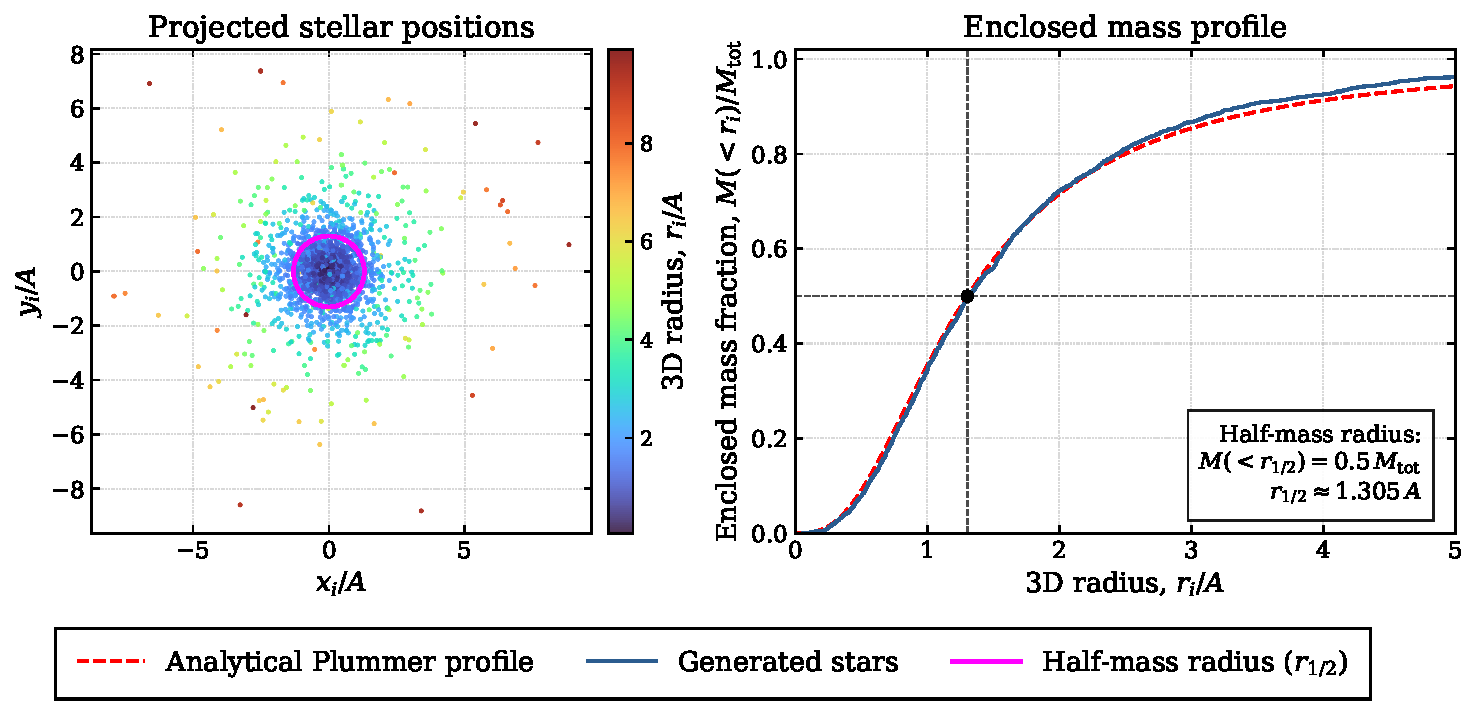
\includegraphics[width=\textwidth]{./plots/cluster_initial_positions_eng.pdf}
	\caption[Initial spatial distribution of the stellar cluster]{Three-dimensional distribution of the initial positions of stars generated according to the Plummer model. ($N = 2000$, $\clusterRadius = 1.0$)}
	\label{fig:initial-positions}
\end{figure}
\subsection{Velocity Distribution}
\label{subsec:velocita-iniziali}
Once the initial positions have been determined, the velocities of individual stars are generated as a function of their distance $r_i$ from the cluster centre. For each star, the local escape velocity is first calculated:
\begin{equation}
	\escapeVelocity(r_i)=\sqrt{-2\potentialPhi(r_i)}
	=\sqrt{\frac{2\gravitationalConstant\totalMass}{\sqrt{r_i^2+\clusterRadius^2}}}
	\label{eq:escape-velocity}
\end{equation}
The velocity magnitude is sampled according to the theoretical distribution predicted by the isotropic Plummer model:
\begin{equation}
	p(\velV_i\mid r_i)\propto \velV_i^2
	\left(1-\frac{\velV_i^2}{\escapeVelocity^2(r_i)}\right)^{7/2}
	\qquad 0\leq \velV_i\leq \escapeVelocity(r_i)
	\label{eq:plummer-speed-distribution}
\end{equation}
This distribution ensures that the initial velocities are lower than the local escape velocity, preventing stars that are initially unbound from the cluster from being generated. To sample from this distribution, the rejection sampling method \cite{devroye1986nonuniform} is used: a candidate velocity magnitude is generated in the interval $[0,\escapeVelocity(r_i)]$ and accepted with a probability proportional to the theoretical distribution. Otherwise, the sample is rejected and generated again.
The velocity magnitude of star $i$ therefore corresponds to the accepted candidate value.
Once the magnitude has been determined, the velocity direction is sampled isotropically in three-dimensional space. The velocity vector of star $i$ is obtained by multiplying the magnitude by a randomly sampled unit direction vector $\hat{\mathbf{n}}_i$:
\begin{equation}
	\mathbf{v}_i=\velV_i\hat{\mathbf{n}}_i
	\label{eq:initial-velocity}
\end{equation}
\begin{figure}[H]
	\centering
	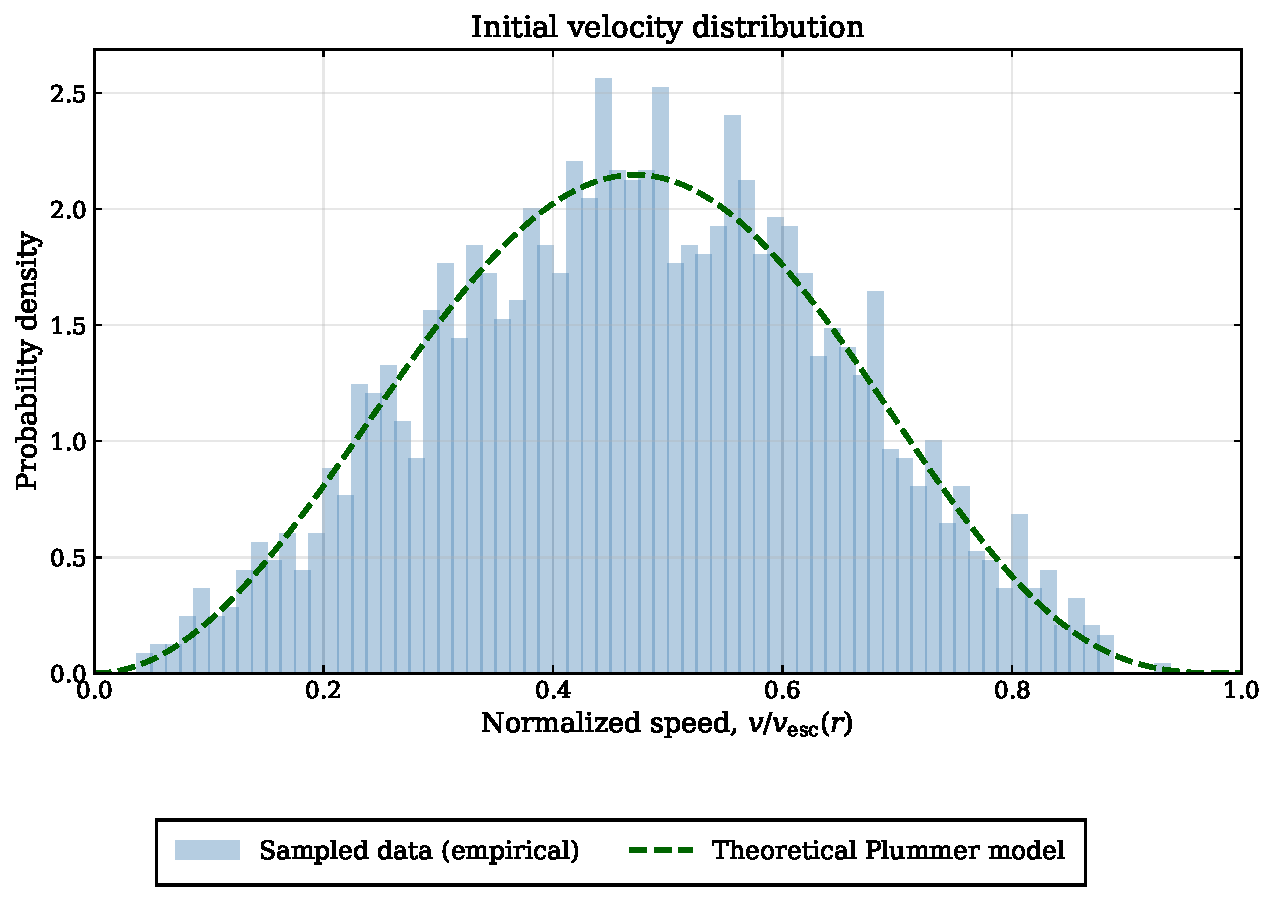
\includegraphics[width=0.85\textwidth]{./plots/cluster_initial_velocities_eng.pdf}
	\caption[Comparison of the initial velocity distributions]{Distributions of velocity magnitudes normalised by the local escape velocity.\\($\numberOfStars = 2000$, $\clusterRadius = 1.0$)}
	\label{fig:velocity-distribution-comparison}
\end{figure}
\subsection{Virial Equilibrium Condition}
\label{subsec:equilibrio-viriale}
To evaluate the initial dynamical equilibrium of the cluster, the total kinetic energy $\totalCineticEnergy$ and the gravitational potential energy $\totalPotentialEnergy$ are considered \cite{ciotti2021}. The kinetic energy is given by the sum of the contributions from all stars:
\begin{equation}
	\totalCineticEnergy = \sum_{i=1}^{N}\frac{1}{2}m_i\left\|\velV_i\right\|^2
	\label{eq:kinetic-energy}
\end{equation}
The gravitational potential energy is obtained by summing the interactions between all pairs of stars:
\begin{equation}
	\totalPotentialEnergy = -\sum_{i=1}^{N-1}\sum_{j=i+1}^{N}
	\frac{\gravitationalConstant m_i m_j}{\left\|\mathbf{x}_i-\mathbf{x}_j\right\|}
	\label{eq:gravitational-potential-energy}
\end{equation}
For a self-gravitating system in virial equilibrium, the two energies satisfy the relation:
\begin{equation}
	2\totalCineticEnergy+\totalPotentialEnergy=0
	\label{eq:virial-theorem}
\end{equation}
The virial ratio makes it possible to quantify the deviation from this condition:
\begin{equation}
	Q=\frac{2\totalCineticEnergy}{|\totalPotentialEnergy|}
	\label{eq:virial-ratio}
\end{equation}
The value $Q=1$ corresponds to virial equilibrium.
\subsection{Velocity Rescaling}
\label{subsec:riscalamento-velocita}
In the continuous Plummer model, the theoretical velocity distribution is consistent with the virial equilibrium condition described in Section~\ref{subsec:equilibrio-viriale}, which is satisfied in the limit of an infinite number of stars ($N\rightarrow\infty$). In simulations, however, the number of stars is finite, and random sampling can result in a kinetic energy that does not exactly satisfy this condition.\\ To correct this deviation, the velocities are multiplied by a common factor $\velocityRescalingFactor$, while the positions of the stars remain unchanged. This procedure does not alter the gravitational potential energy, which depends exclusively on the positions of the particles.
Since kinetic energy is proportional to the square of the velocities, after rescaling we obtain:
\begin{equation}
	\totalCineticEnergy' =
	\velocityRescalingFactor^2 \totalCineticEnergy
	\label{eq:rescaled-kinetic-energy}
\end{equation}
By imposing that the final virial ratio is $\virialRatio'=1$, the rescaling factor can be derived from the energies calculated before the correction:
\begin{equation}
	\velocityRescalingFactor =
	\sqrt{\frac{|\totalPotentialEnergy|}
		{2\totalCineticEnergy}}
	=
	\frac{1}{\sqrt{\virialRatio}}
	\label{eq:velocity-rescaling-factor}
\end{equation}
\begin{figure}[H]
	\centering
	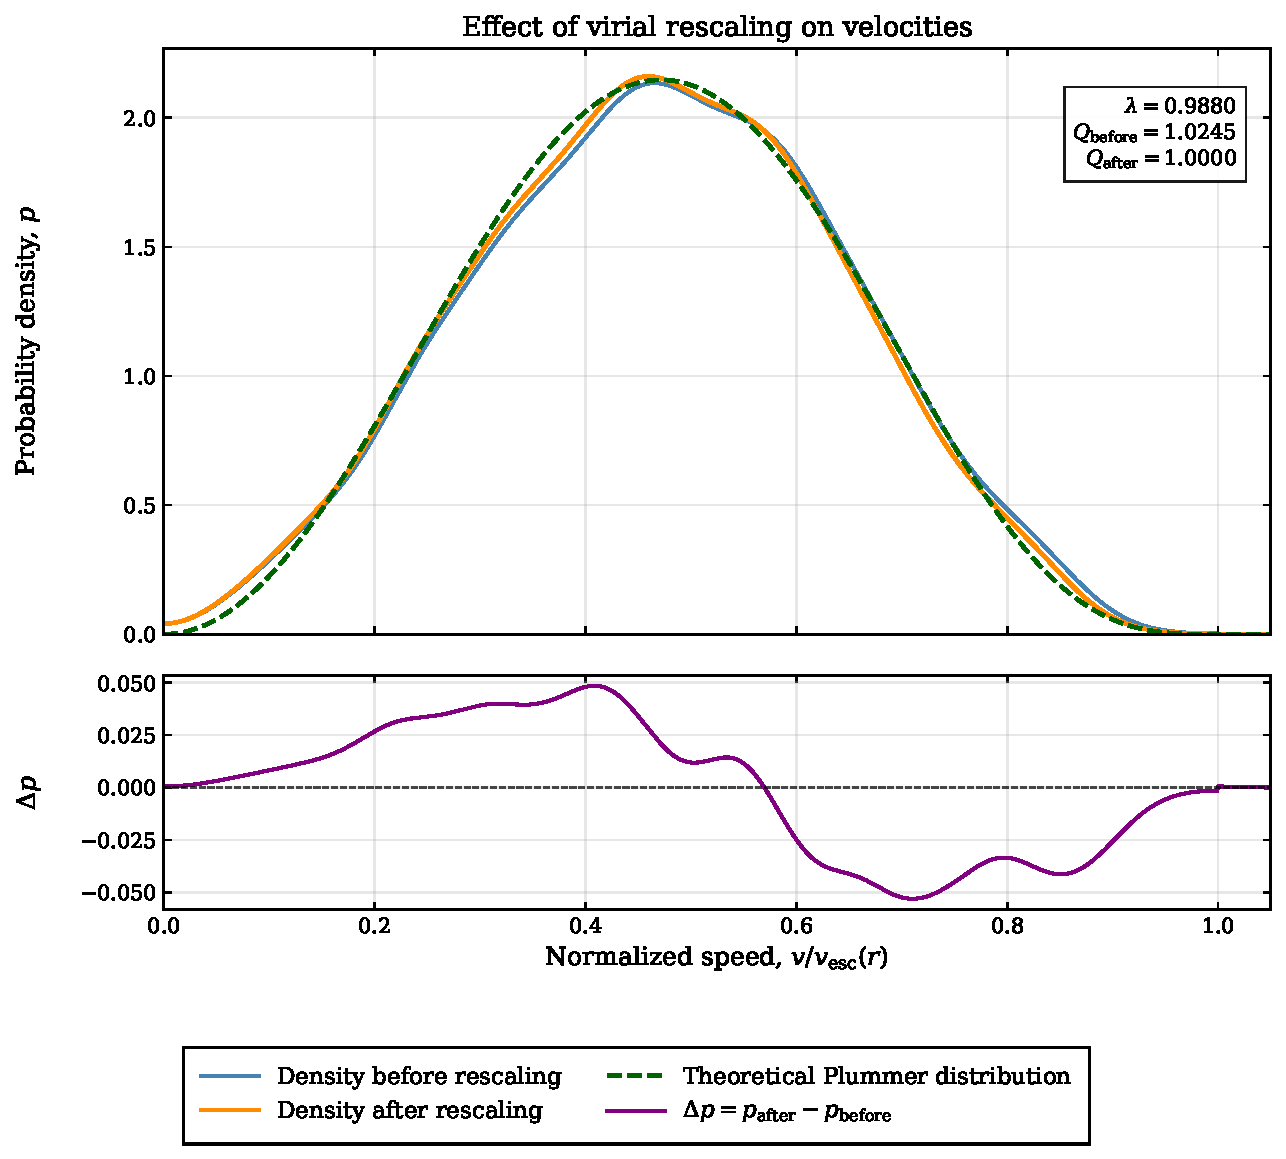
\includegraphics[width=0.85\textwidth]{./plots/cluster_velocity_rescaling_eng.pdf}
	\caption[Effect of virial rescaling on velocities]{Distributions of velocity magnitudes normalised before and after rescaling.\\($\numberOfStars = 2000$, $\clusterRadius = 1.0$)}
	\label{fig:velocity-rescaling}
\end{figure}
\section{Evolution and Orbital Dynamics}
\label{sec:evoluzione-ammasso}
The evolution of the stellar cluster is described through the gravitational interaction between the stars and the external galactic potential, which determines its orbital dynamics and evolution over time.
\subsection{Galactic Plummer Potential}
\label{subsec:plummer-galattico}
The Plummer model \cite{plummer1911}, already introduced in Section~\ref{subsec:plummer} to model the mass distribution of the stellar cluster, is also adopted to describe the gravitational potential of the galaxy. In this case, the model represents the external gravitational field in which the cluster evolves and is expressed as a function of the distance $\galaxyDistance$ from the galactic centre:
\begin{equation}
	\potentialPhi_{\mathrm{gal}}(\galaxyDistance) =
	-\frac{\gravitationalConstant \galaxyMass}
	{\sqrt{\galaxyDistance^2+\galaxyRadius^2}}
	\label{eq:galactic-plummer-potential}
\end{equation}
The parameter $\galaxyRadius$ represents the scale length of the galactic model and characterises its extent.
The adopted form avoids the singularity of the potential at the centre, which occurs in the case of a point mass.\\
Starting from the potential defined in Equation~\eqref{eq:galactic-plummer-potential}, the gravitational acceleration exerted by the galaxy is obtained by calculating the negative gradient of the potential:
\begin{equation}
	\mathbf{a}_{\mathrm{gal}}(\mathbf{R}) =
	-\frac{\gravitationalConstant \galaxyMass}
	{(\galaxyDistance^2+\galaxyRadius^2)^{3/2}}\mathbf{R}
	\label{eq:galactic-plummer-acceleration}
\end{equation}
\begin{figure}[H]
	\centering
	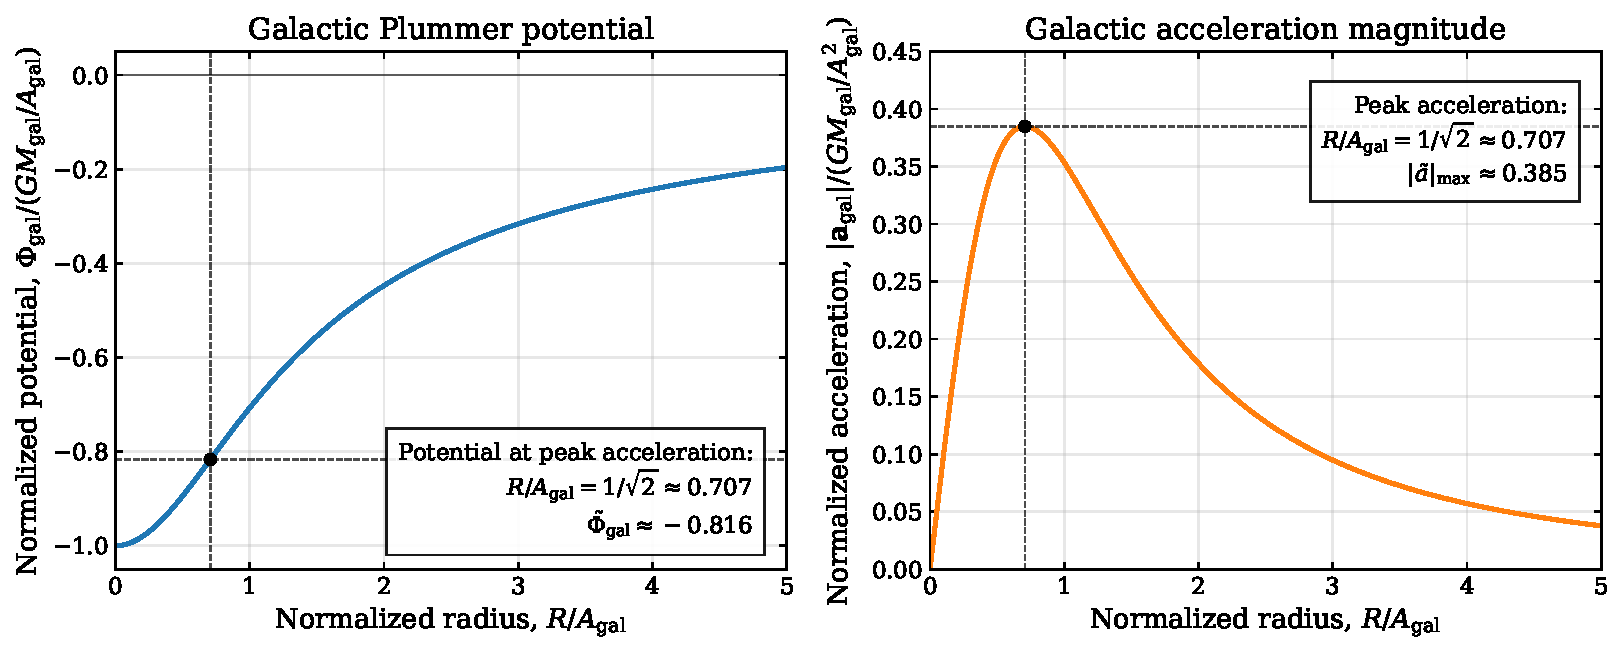
\includegraphics[width=\textwidth]{plots/galactic_plummer_potential_eng.pdf}
	\caption[Potential and acceleration of the galactic Plummer model]{Gravitational potential and acceleration magnitude of the galactic Plummer model.\\($G = 1.0$, $M_{\mathrm{gal}} = 2000.0$, $A_{\mathrm{gal}} = 10.0$)}
	\label{fig:galactic-plummer}
\end{figure}
\subsection{Equations of Motion}
\label{subsec:equazioni-moto}
The evolution of the stellar cluster is described by Newton's equations for a system of gravitationally interacting particles \cite{goldstein2002}. Letting $\mathbf{x}_i$ denote the position of star $i$ and $m_i$ its mass, the equations of motion are:
\begin{equation}
	\frac{d\mathbf{x}_i}{dt} = \mathbf{v}_i
	\qquad
	\frac{d\mathbf{v}_i}{dt} = \mathbf{a}_i
	\label{eq:equations-of-motion}
\end{equation}
To regularise the gravitational potential during close encounters between stars, a softening parameter $\softeningLength$ is introduced. The potential energy of interaction between two stars $i$ and $j$ therefore becomes:
\begin{equation}
	U_{ij}=-\frac{\gravitationalConstant m_i m_j}
	{\sqrt{\left\|\mathbf{x}_i-\mathbf{x}_j\right\|^2+\softeningLength^2}}
	\label{eq:softened-potential}
\end{equation}
The internal contribution, accounting for the softening parameter, is expressed as:
\begin{equation}
	\mathbf{a}_{i,\mathrm{int}} =
	-G\sum_{\substack{j=1\\j\neq i}}^N
	m_j
	\frac{\mathbf{x}_i-\mathbf{x}_j}
	{\left(\left\|\mathbf{x}_i-\mathbf{x}_j\right\|^2+\softeningLength^2\right)^{3/2}}
	\label{eq:internal-gravitational-acceleration}
\end{equation}
The total acceleration is therefore the sum of the internal contribution and the galactic contribution defined in Section~\ref{subsec:plummer-galattico}:
\begin{equation}
	\mathbf{a}_i =
	\mathbf{a}_{i,\mathrm{int}} +
	\mathbf{a}_{\mathrm{gal}}(\mathbf{x}_i)
	\label{eq:total-acceleration}
\end{equation}
This formulation makes it possible to describe simultaneously the internal dynamics of the cluster and its response to the external gravitational field. Mutual interactions determine the evolution of the stellar structure, while the galactic potential influences the overall motion of the cluster and can promote the loss of stars that are no longer gravitationally bound to its internal component \cite{binneytremaine2008}.
\subsection{Initial Orbital Parameters}
\label{subsec:parametri-orbitali-iniziali}
The initial orbit of the stellar cluster is defined through the semi-major axis $\semiMajorAxis$ and the eccentricity $\orbitEccentricity$. These parameters determine the maximum distance $R_{\mathrm{apo}}$ and the minimum distance $R_{\mathrm{peri}}$ from the galactic centre:
\begin{equation}
	R_{\mathrm{apo}} = \semiMajorAxis(1+\orbitEccentricity)
	\qquad
	R_{\mathrm{peri}} = \semiMajorAxis(1-\orbitEccentricity)
	\label{eq:orbital-extrema}
\end{equation}
The cluster is initially placed at a distance $R_{\mathrm{apo}}$, with a velocity perpendicular to the radial direction. Its magnitude is determined using the conservation of specific mechanical energy and specific angular momentum \cite{goldstein2002}:
\begin{equation}
	E = \frac{\velV^2}{2} + \potentialPhi_{\mathrm{gal}}(R)
	\qquad
	L = R v_{\mathrm{t}}
	\label{eq:orbital-conservation}
\end{equation}
where $R$ is the distance from the galactic centre, $\velV$ is the velocity magnitude and $v_{\mathrm{t}}$ is the tangential component. At apocentre and pericentre, the velocity is entirely tangential. Equating the energy at the two points and imposing conservation of angular momentum gives:
\begin{equation}
	L^2 =
	\frac{2\left[
		\potentialPhi_{\mathrm{gal}}(R_{\mathrm{apo}})
		-\potentialPhi_{\mathrm{gal}}(R_{\mathrm{peri}})
		\right]}
	{R_{\mathrm{peri}}^{-2}-R_{\mathrm{apo}}^{-2}}
	\label{eq:orbital-angular-momentum}
\end{equation}
The initial velocity at apocentre is therefore:
\begin{equation}
	v_{\mathrm{apo}} = \frac{L}{R_{\mathrm{apo}}}
	\label{eq:orbital-apocenter-velocity}
\end{equation}
The velocity calculated in this way is assigned to all stars in the cluster, superimposed on their individual motions. Figure~\ref{fig:confronto-eccentricita} shows, using OVITO \cite{stukowski2010}, the evolution of the cluster for two different orbital eccentricities.
\begin{figure}[H]
	\centering
	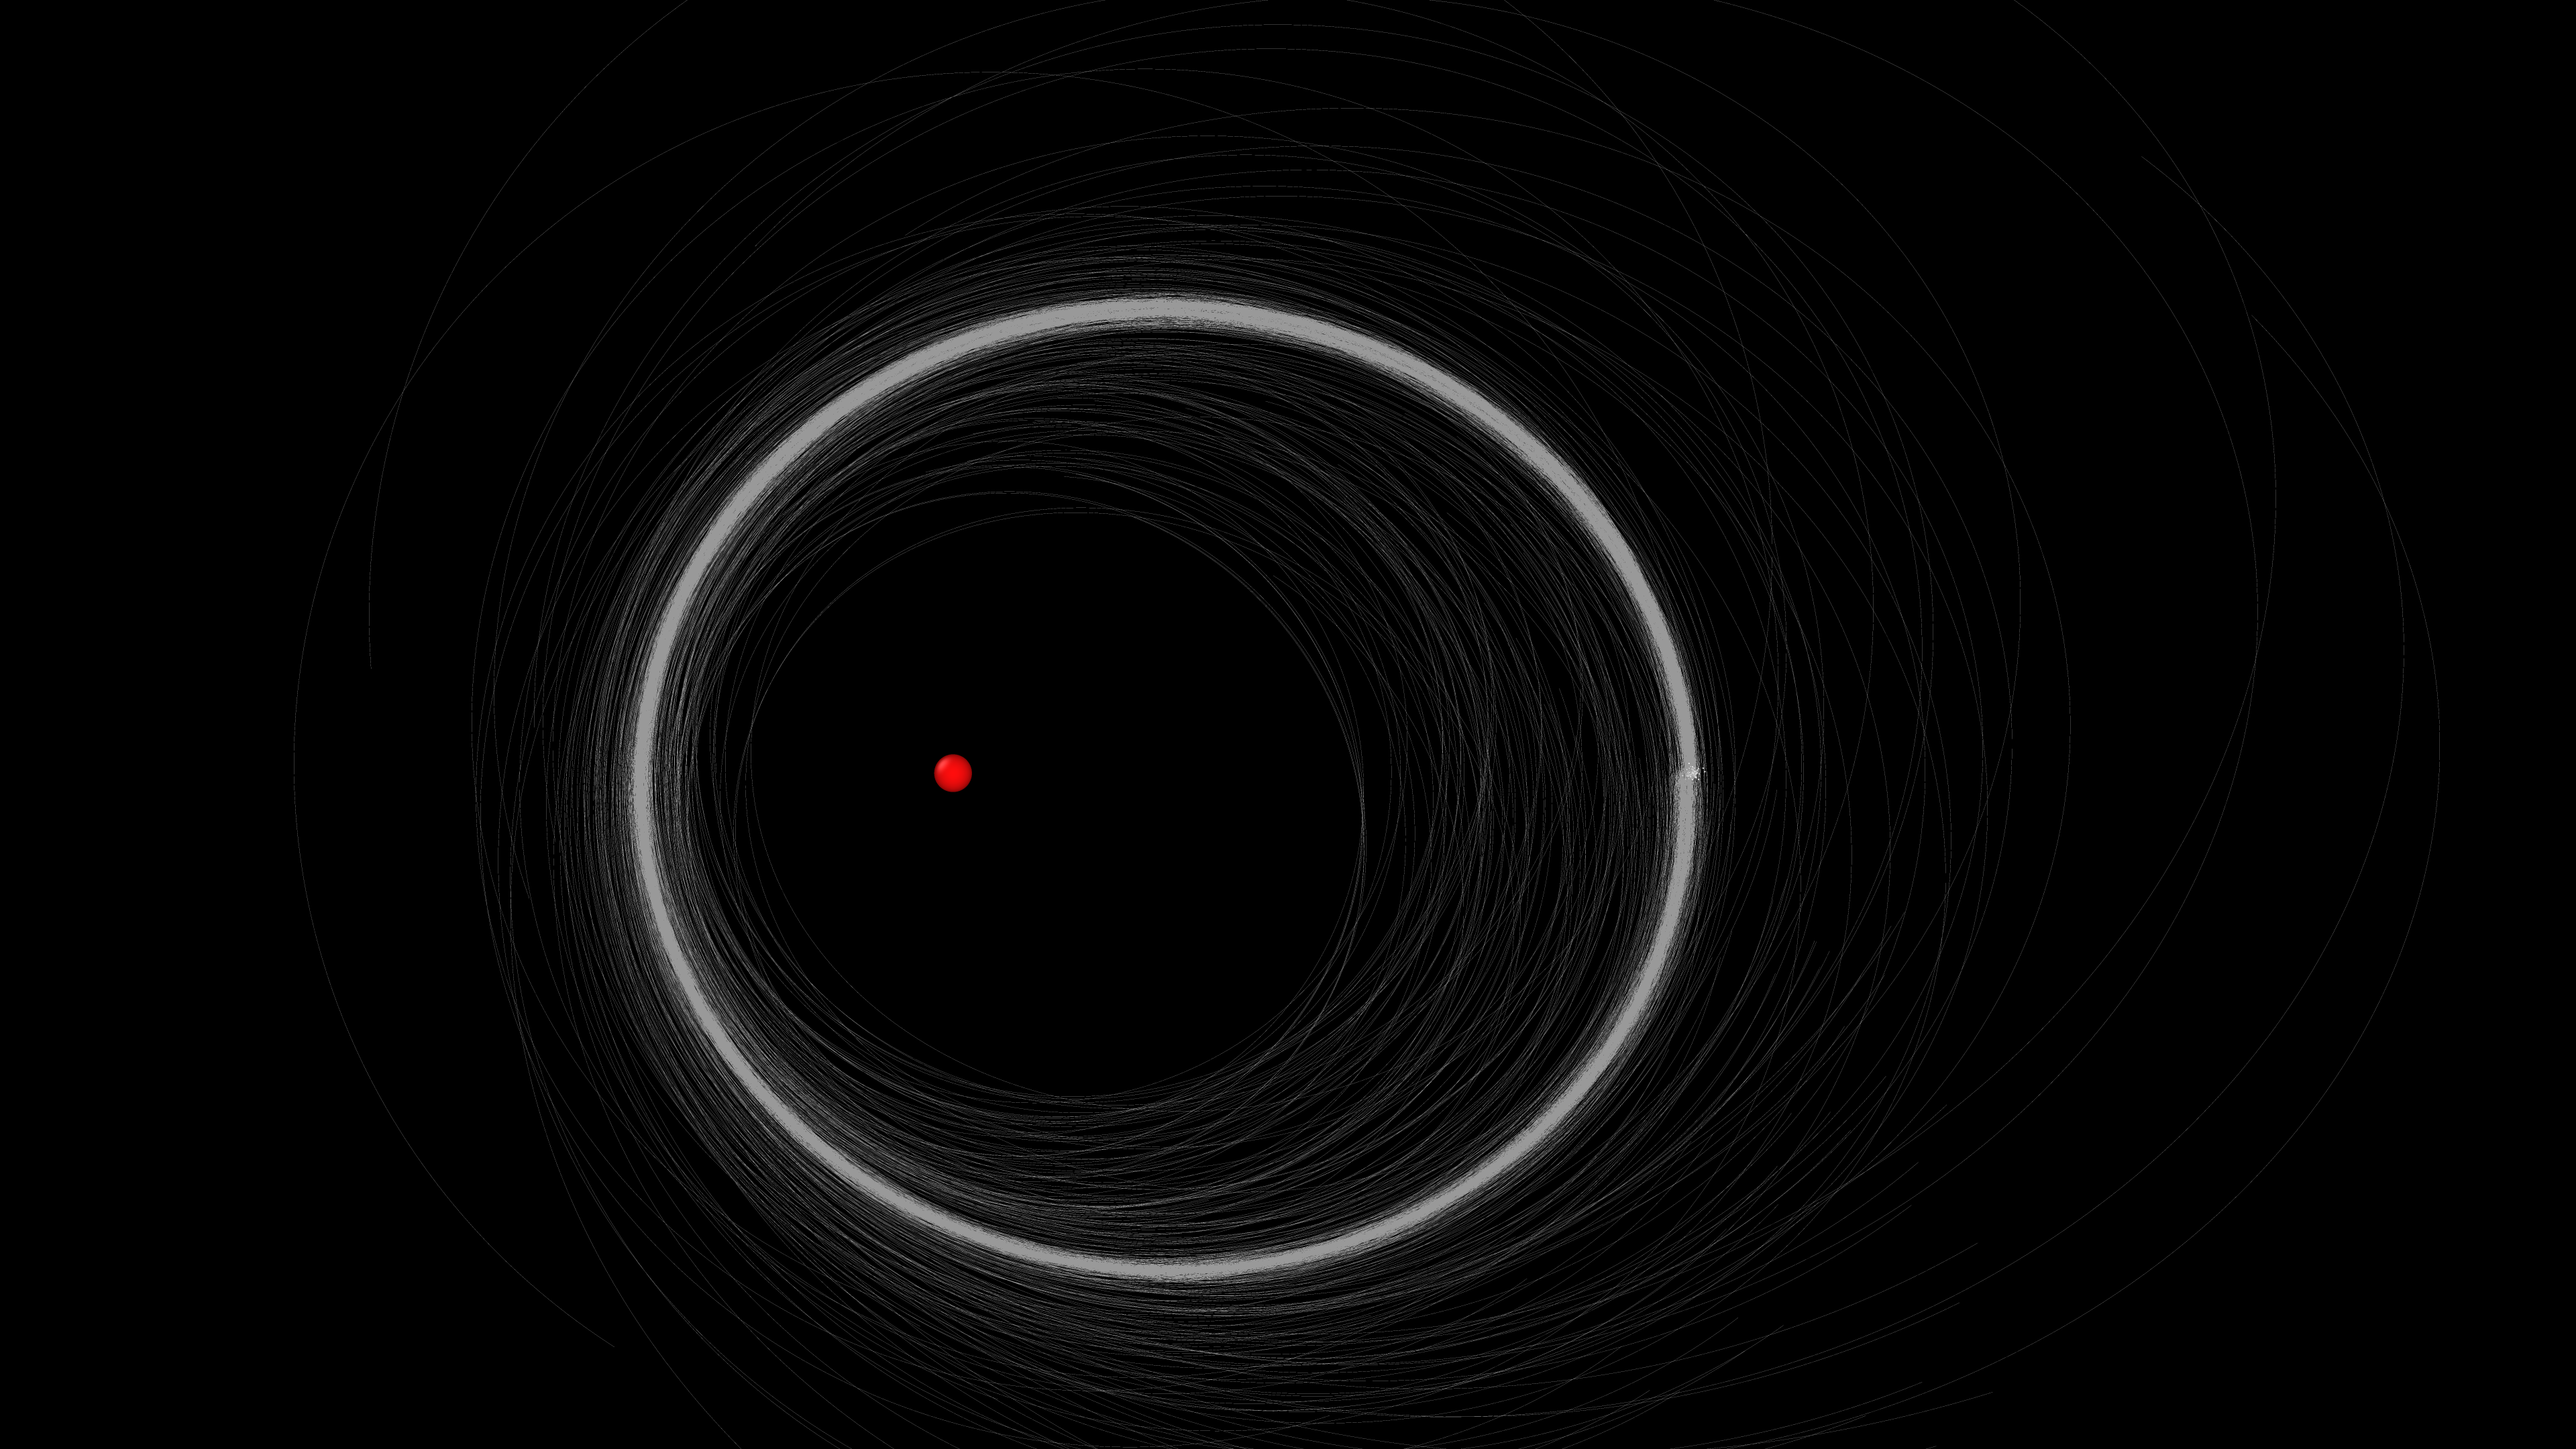
\includegraphics[width=0.48\textwidth]{./images/ovito_e03.png}
	\hfill
	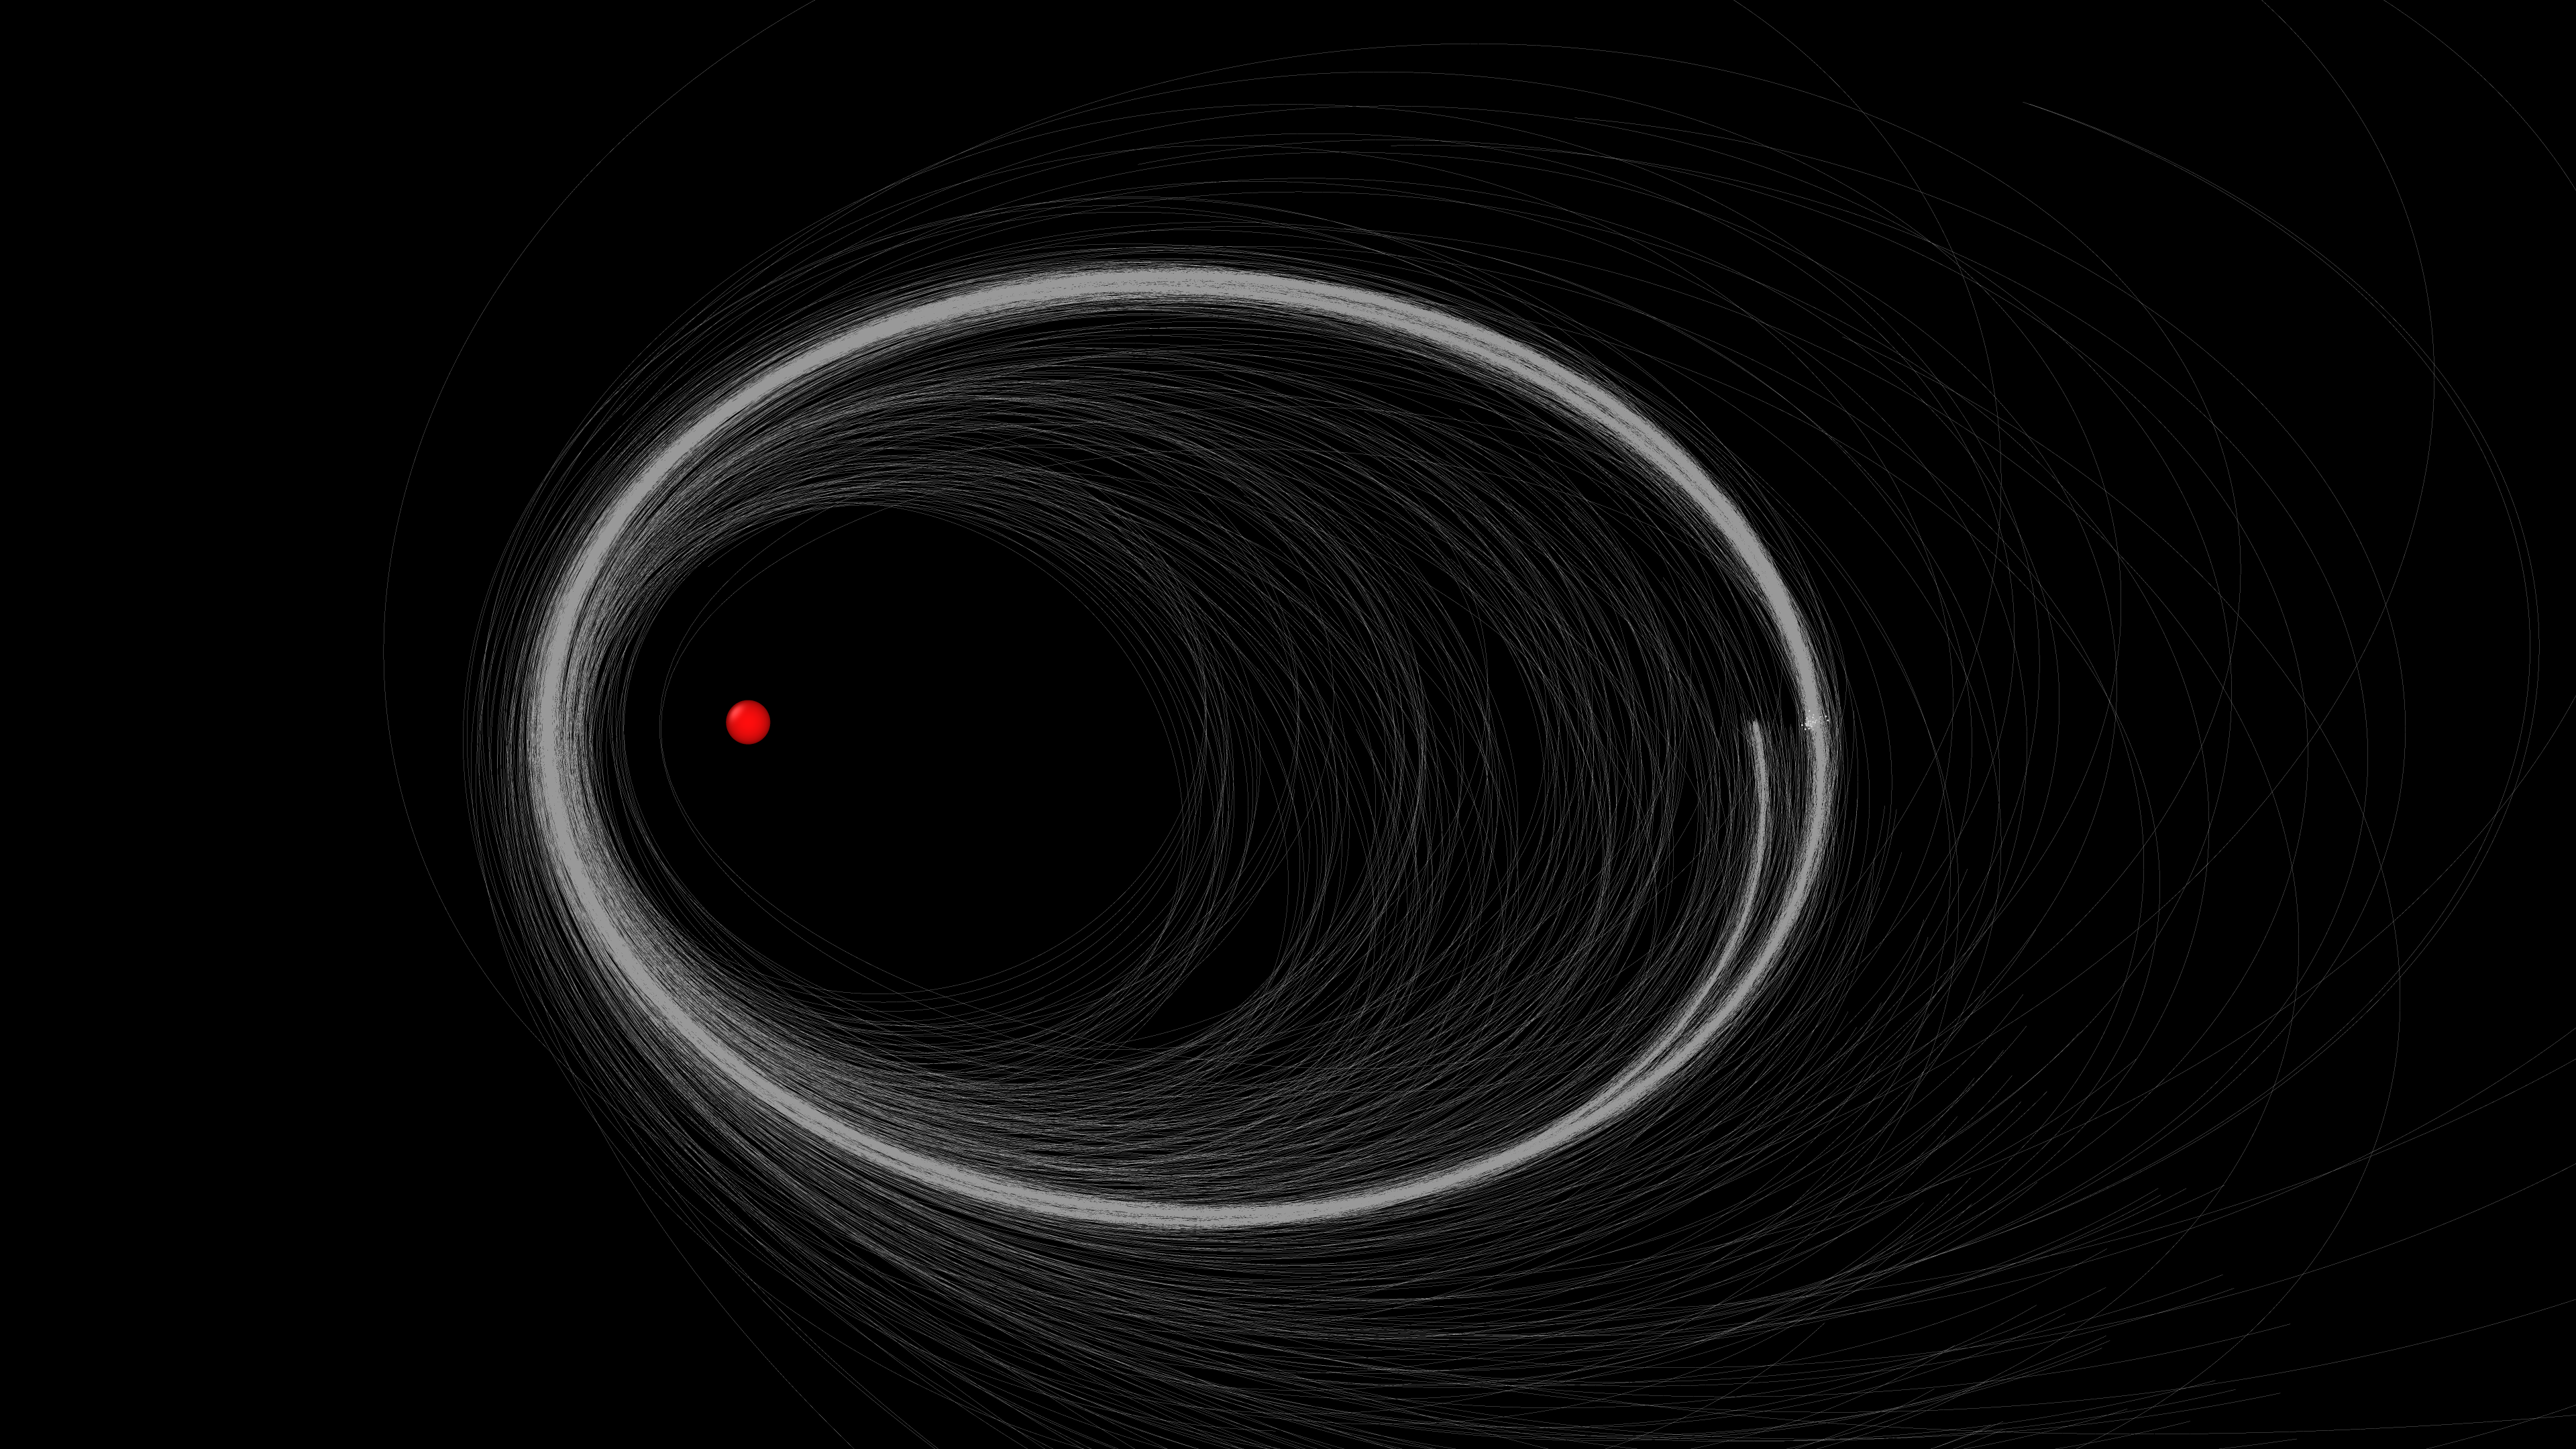
\includegraphics[width=0.48\textwidth]{./images/ovito_e06.png}
	\caption{Evolution of the same stellar cluster after two orbits, with eccentricity $e = 0.3$ (left) and $e = 0.6$ (right). The white trajectories trace the movement of the stars, and the red dot indicates the galactic centre.\\ ($\numberOfStars = 400$, $\clusterRadius = 1.0$, $\galaxyMass = 2000.0$, $\galaxyRadius = 10.0$, $\gravitationalConstant = 1.0$, $\softeningLength = 0.01$, $\semiMajorAxis = 300.0$, $\deltat = 0.005$, \emph{leapfrog})}
	\label{fig:confronto-eccentricita}
\end{figure}
\subsection{Numerical Integration}
\label{subsec:integrazione-numerica}
The evolution of the system is calculated using the \emph{leapfrog} numerical integrator, a second-order symplectic method commonly used in long-term dynamical simulations \cite{quinn1997timestepping}.
Letting $\deltat$ denote the time step, the method updates positions and velocities in three stages: first, it advances the stars by half a time step using their current velocities; it then updates the velocities by one full time step using the accelerations calculated at the intermediate positions; finally, it completes the displacement of the stars with a further half-step.
The update equations are:
\begin{align}
	\mathbf{x}_{i}^{n+1/2}
	&= \mathbf{x}_{i}^{n}
	+ \frac{\deltat}{2}\mathbf{v}_{i}^{n}\\
	\mathbf{v}_{i}^{n+1}
	&= \mathbf{v}_{i}^{n}
	+ \deltat\,\mathbf{a}_{i}^{n+1/2}\\
	\mathbf{x}_{i}^{n+1}
	&= \mathbf{x}_{i}^{n+1/2}
	+ \frac{\deltat}{2}\mathbf{v}_{i}^{n+1}
	\label{eq:leapfrog-update}
\end{align}
In this work, a time step of $\deltat=0.005$ is adopted for all simulations, which are run until the final time $\simulationEndTime=700.0$.\\ To verify the behaviour of the numerical integration, the relative variation of the total energy with respect to its initial value is monitored. Letting $E(t)$ denote the total energy of the system at time $t$ and $E_0=E(0)$ its initial value, this variation is defined as:
\begin{equation}
	\delta_E(t)=\frac{\Delta E(t)}{E_0}
	=\frac{E(t)-E(0)}{E(0)}
	\label{eq:energy-drift}
\end{equation}
This quantity is dimensionless and makes it possible to evaluate the relative deviation of the energy from its initial value.
As an indicative reference, a maximum deviation of $\max_t|\delta_E(t)|\lesssim10^{-3}$ can be considered small; in the case shown in Figure~\ref{fig:energy-drift}, the deviation takes values between approximately $-5\times10^{-3}$ and $1.25\times10^{-2}$, which are considered acceptable.
\begin{figure}[H]
	\centering
	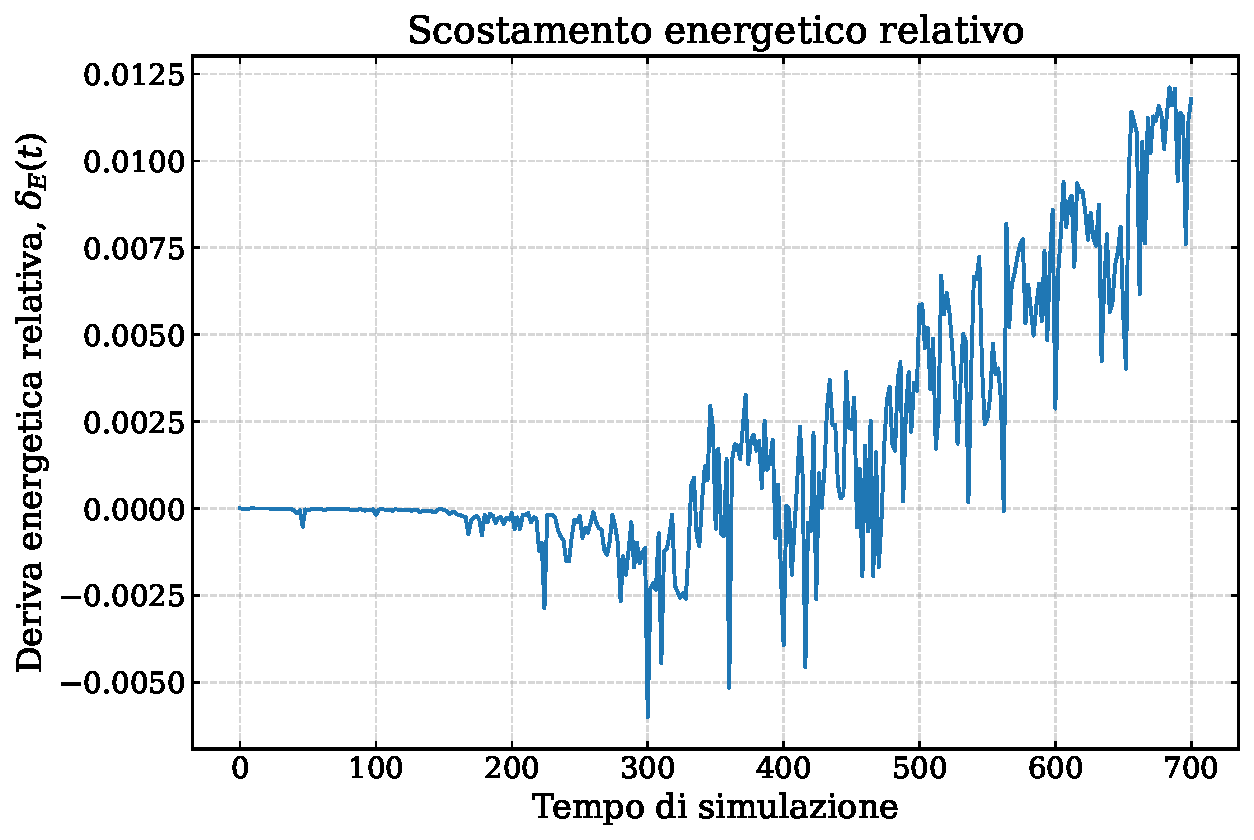
\includegraphics[width=0.8\textwidth]{./plots/energy_drift.pdf}
	\caption{Relative energy drift $\delta_E(t)$ as a function of simulation time.\\($\numberOfStars = 400$, $\clusterRadius = 1.0$, $\galaxyMass = 2000.0$, $\galaxyRadius = 10.0$, $\gravitationalConstant = 1.0$, $\softeningLength = 0.01$, $\semiMajorAxis = 300.0$, $\orbitEccentricity = 0.6$, $\deltat = 0.005$, $\simulationEndTime = 700.0$, \emph{leapfrog})}
	\label{fig:energy-drift}
\end{figure}
\subsection{Identifying Stars Bound to the Cluster}
\label{subsec:stelle-legate}
A star is considered gravitationally bound to the cluster if its specific mechanical energy is negative. We therefore define the set of bound stars $\boundSet$ as:
\begin{equation}
	\boundSet = \left\{i \mid \specificEnergy < 0\right\},
	\qquad \specificEnergy = \kineticEnergy + \specificPotential
	\label{eq:bound-stars}
\end{equation}
where $\kineticEnergy$ and $\specificPotential$ are, respectively, the specific kinetic energy and the specific gravitational potential of star $i$.
The specific kinetic energy is calculated with respect to the velocity of the centre of mass of the bound component:
\begin{equation}
	\kineticEnergy = \frac{1}{2}
	\left\|\mathbf{v}_i-\boundCenterVelocity\right\|^2
	\label{eq:stellar-kinetic-energy}
\end{equation}
where $\mathbf{v}_i$ is the velocity of star $i$ and $\boundCenterVelocity$ is the velocity of the centre of mass of the bound stars, defined in Section~\ref{subsec:centro-massa-legato}.
The specific gravitational potential of star $i$ is calculated by summing the contributions from all the other stars belonging to $\boundSet$:
\begin{equation}
	\specificPotential = -\gravitationalConstant \sum_{\substack{j \in \boundSet \\ j \neq i}}
	\frac{m_j}{\left\|\mathbf{x}_i-\mathbf{x}_j\right\|}
	\label{eq:stellar-potential}
\end{equation}
where $\gravitationalConstant$ is the universal gravitational constant, $m_j$ is the mass of star $j$, and $\mathbf{x}_i$ and $\mathbf{x}_j$ are the positions of the stars.
The calculation of the specific energy therefore depends on the set $\boundSet$, which determines both the centre-of-mass velocity used as the reference for calculating the kinetic energy and the stars contributing to the gravitational potential. To resolve this mutual dependence, the selection is performed iteratively, updating $\boundSet$ and the velocity of its centre of mass at each step:
\begin{enumerate}
	\item The star with the lowest gravitational potential is identified, and the eleven nearest stars are selected. Their mass-weighted mean velocity provides an initial estimate of the centre-of-mass velocity.
	\item $\boundSet$ is initialised with all the stars in the cluster, and the specific energies are calculated. The stars with negative energy form the new set $\boundSet$.
	\item The energies are recalculated using the updated centre-of-mass velocity and the potential generated only by the stars belonging to the new set $\boundSet$. The procedure is repeated until $\boundSet$ no longer changes, for a maximum of ten iterations. If at most three stars remain, no bound component is identified.
\end{enumerate}
\subsection{Centre of Mass of the Stars Bound to the Cluster}
\label{subsec:centro-massa-legato}
After identifying the set $\boundSet$ of bound stars, according to the procedure described in Section~\ref{subsec:stelle-legate}, the position and velocity of the centre of mass of the bound component are calculated as mass-weighted averages:
\begin{equation}
	\boundCenterPosition =
	\frac{\displaystyle\sum_{i\in\boundSet}m_i\mathbf{x}_i}
	{\displaystyle\sum_{i\in\boundSet}m_i}
	\label{eq:com-bound-position}
\end{equation}
The centre-of-mass velocity is calculated in the same way:
\begin{equation}
	\boundCenterVelocity =
	\frac{\displaystyle\sum_{i\in\boundSet}m_i\mathbf{v}_i}
	{\displaystyle\sum_{i\in\boundSet}m_i}
	\label{eq:com-bound-velocity}
\end{equation}
In these expressions, $m_i$, $\mathbf{x}_i$ and $\mathbf{v}_i$ denote, respectively, the mass, position and velocity of star $i$.
\subsection{Bound Mass Fraction}
\label{subsec:frazione-massa-legata}
The bound mass fraction expresses the portion of the total mass that remains gravitationally bound to the cluster. Letting $m_i$ denote the mass of star $i$, the bound mass is:
\begin{equation}
	\boundMass = \sum_{i\in\boundSet}m_i
	\label{eq:bound-mass}
\end{equation}
The bound mass fraction is obtained by dividing this quantity by the total mass $\totalMass$ of all the stars:
\begin{equation}
	\boundMassFraction =
	\frac{\boundMass}{\totalMass}
	\label{eq:bound-mass-fraction}
\end{equation}
The value $\boundMassFraction=1.0$ corresponds to 100\% of the initial mass still gravitationally bound to the cluster, whereas a value of zero indicates that no bound mass remains.
The bound mass fraction $\boundMassFraction$ is therefore a suitable quantity for describing the evolution of the gravitationally bound mass of the stellar cluster over time.
\subsection{Half-Mass Radius}
\label{subsec:raggio-meta-massa}
The half-mass radius indicates the distance from the centre of mass within which half of the bound mass is contained. For each star belonging to $\boundSet$, the distance from the centre of mass is calculated:
\begin{equation}
	\stellarDistance =
	\left\|\mathbf{x}_i-\boundCenterPosition\right\|
	\qquad \forall i\in\boundSet
	\label{eq:stellar-distance}
\end{equation}
The stars are then sorted by increasing distance, and the cumulative mass of the bound component is calculated. The mass contained within a distance $r$, denoted by $M_{\mathrm{bound}}(<r)$, is:
\begin{equation}
	M_{\mathrm{bound}}(<r) = \sum_{\substack{i\in\boundSet\\d_i\leq r}}m_i
	\label{eq:cumulative-bound-mass}
\end{equation}
The half-mass radius is the minimum distance at which the cumulative mass reaches at least half of the bound mass:
\begin{equation}
	\halfMassRadius = \min\left\{r : M_{\mathrm{bound}}(<r)\geq\frac{\boundMass}{2}\right\}
	\label{eq:half-mass-radius}
\end{equation}
If no gravitationally bound component is identified, the half-mass radius is set to zero.
The half-mass radius $\halfMassRadius$ is therefore a suitable quantity for describing the evolution of the spatial distribution of the bound mass over time.%
